\section{Results}
The results of the experiments are shown in figure \ref{fig:experiment}. Blue lines represent the results of the \textit{KD-tree} and the other one (orange) of the \textit{RKD-tree}. Now I am going to explain the meaning of this results, parameter by parameter.
\begin{itemize}
      \item $\mathbf{n}$. As you can see in figure \ref{fig:n_times}, when $n \approx 10000$, more or less a half of the total data, the \textit{RKD-tree} starts to last more time than the \textit{KD-tree}. The accuracy (successful search rate, figure \ref{fig:n_acc}) in this point is roughly between 0.6 and 0.7. As I explained in section \ref{sec:summary}, the authors said that \textit{RKD-tree} can reach a 0.88 accuracy with 3-times speed-up, with $n = 1000$. In my case this is not possible. For the rest of the experiments I fixed $n$ to $8000$ since, with it, I obtained an acceptable accuracy with an acceptable search time.
      \item $\mathbf{m}$. In figure \ref{fig:m_times} we can see that increasing the number of trees also increases the search time, but it seems that around $m = 30$ it stabilizes. Regarding the accuracy (figure \ref{fig:m_acc}), it tends to increase, but the randomness of the experiments leads to significant accuracy differences in each iteration, so it is not so clear. Moreover, the construction time of the \textit{RKD-tree} increases linearly (figure \ref{fig:const_times}) because it has to build one \textit{KD-tree} more in each iteration. For the rest of the experiments, I fixed $m$ to $24$ since I achieved the best accuracy with it.
      \begin{figure}[hbtp]
            \centering
            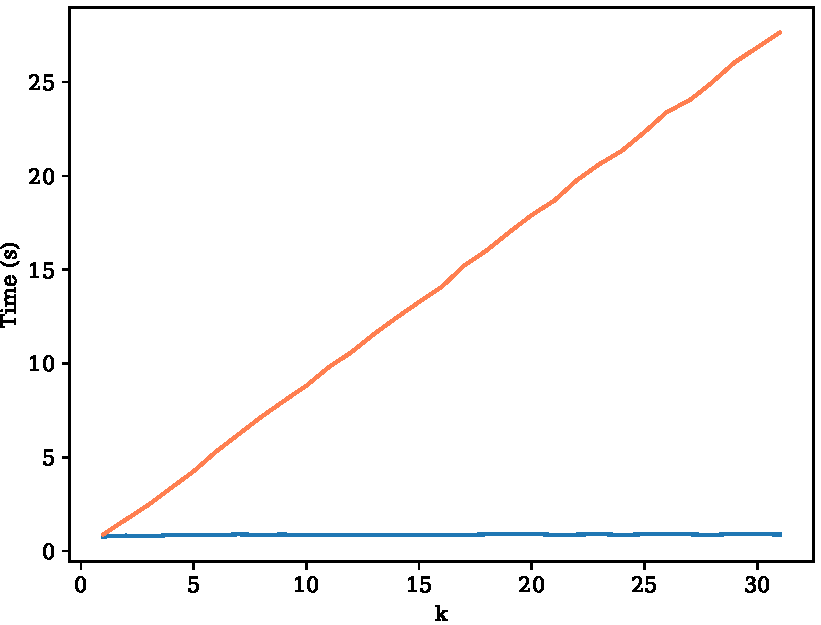
\includegraphics[width=0.45\textwidth]{construct_times.pdf}
            \caption{Construction time}
            \label{fig:const_times}
      \end{figure}
      \item $\mathbf{k}$. As you can see in figure \ref{fig:hv_times}, for the first time, one of the parameters affects the same in both kind of trees. The value of $k$ does not seem to be so relevant when $k > 10$, approximately. When it is lower than that, the performance is really bad, both in time and accuracy. I fixed $k$ to 41 because I achieved the best accuracy with it.
\end{itemize}

The \textit{RKD-tree} with the tunned parameters ($n = 8000, m = 24, k = 41$) leads to 0.6 accuracy with a mean time of 4.189s, while \textit{KD-tree} lasts 4.898s to obtain the nearest point. Also mention that the construction of the \textit{RKD-tree} lasts 20.58s while \textit{KD-tree} lasts $0.889s$.

\begin{figure*}[hbtp]
    \begin{subfigure}[b]{0.45\textwidth}
          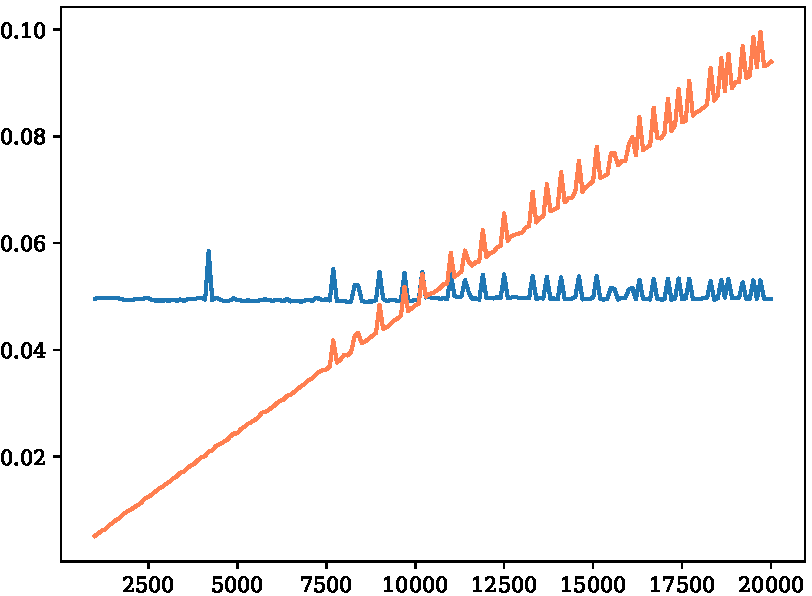
\includegraphics[width=\textwidth]{n_times.pdf}
          \caption{Search time}
          \label{fig:n_times}
    \end{subfigure}
    \hspace{0.05\textwidth}
    \begin{subfigure}[b]{0.45\textwidth}
          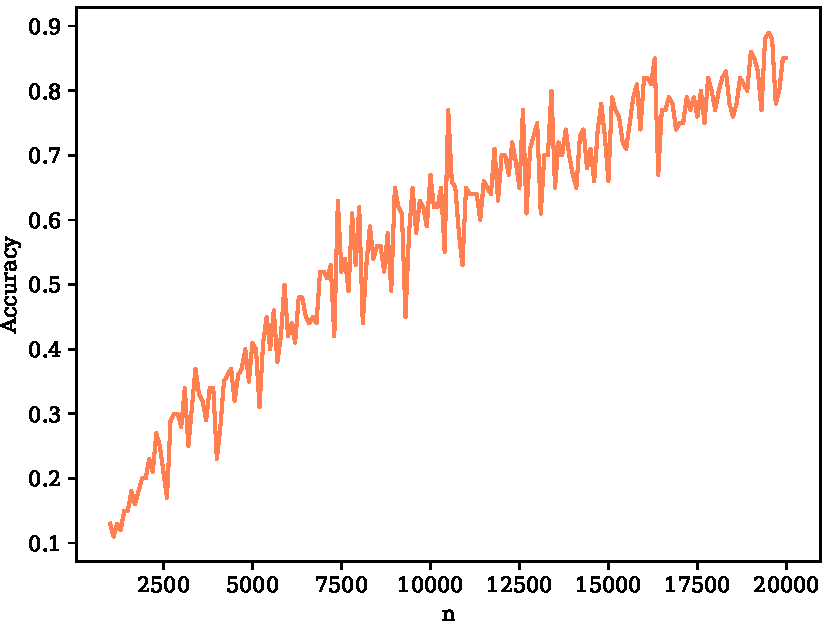
\includegraphics[width=\textwidth]{n_acc.pdf}
          \caption{Accuracy}
          \label{fig:n_acc}
    \end{subfigure}
    \begin{subfigure}[b]{0.45\textwidth}
          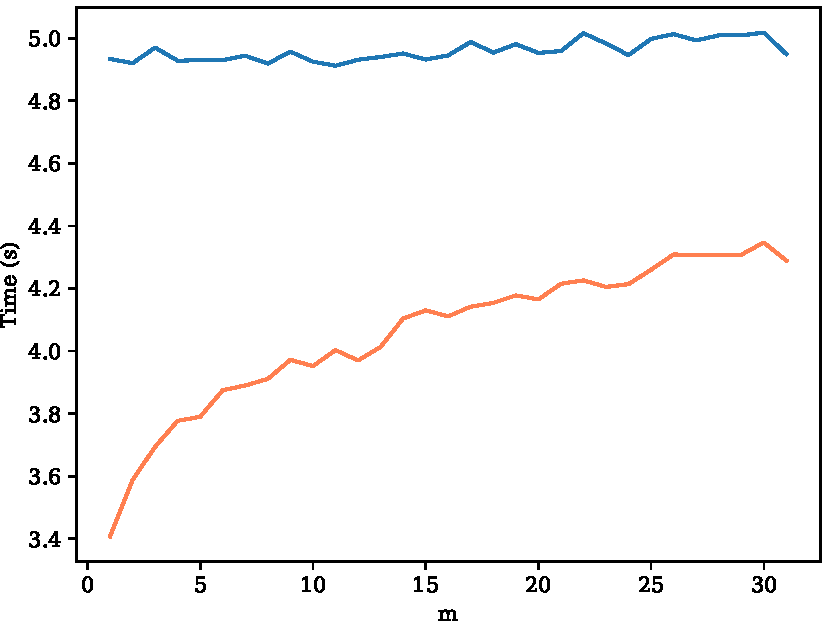
\includegraphics[width=\textwidth]{m_times.pdf}
          \caption{Search time}
          \label{fig:m_times}
    \end{subfigure}
    \hspace{0.05\textwidth}
    \begin{subfigure}[b]{0.45\textwidth}
          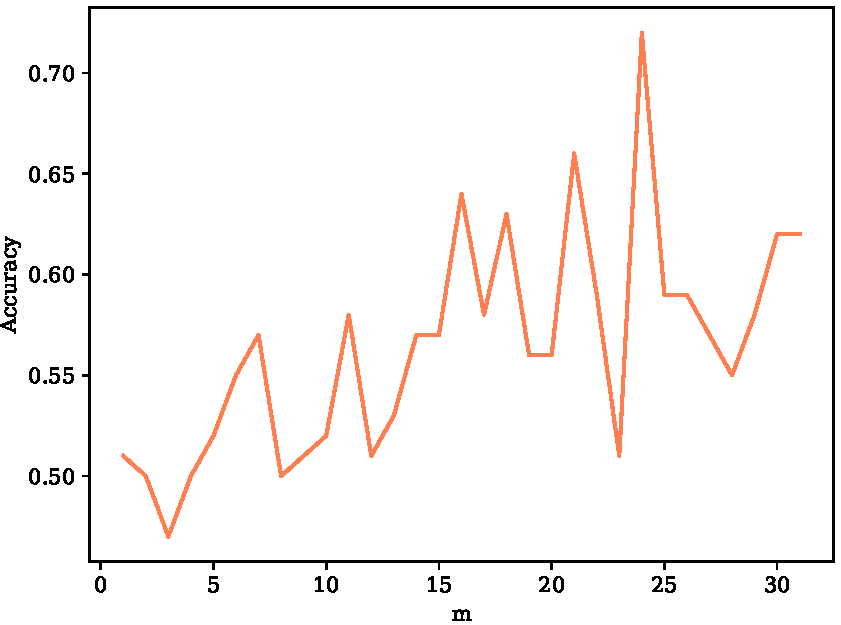
\includegraphics[width=\textwidth]{m_acc.pdf}
          \caption{Accuracy}
          \label{fig:m_acc}
    \end{subfigure}
    \begin{subfigure}[b]{0.45\textwidth}
          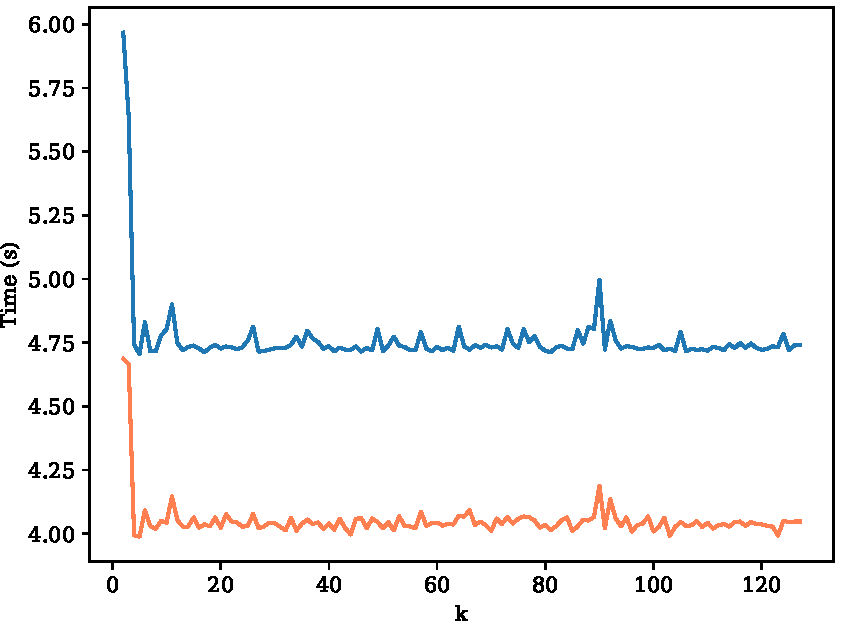
\includegraphics[width=\textwidth]{k_times.pdf}
          \caption{Search time}
          \label{fig:hv_times}
    \end{subfigure}
    \hspace{0.05\textwidth}
    \begin{subfigure}[b]{0.45\textwidth}
          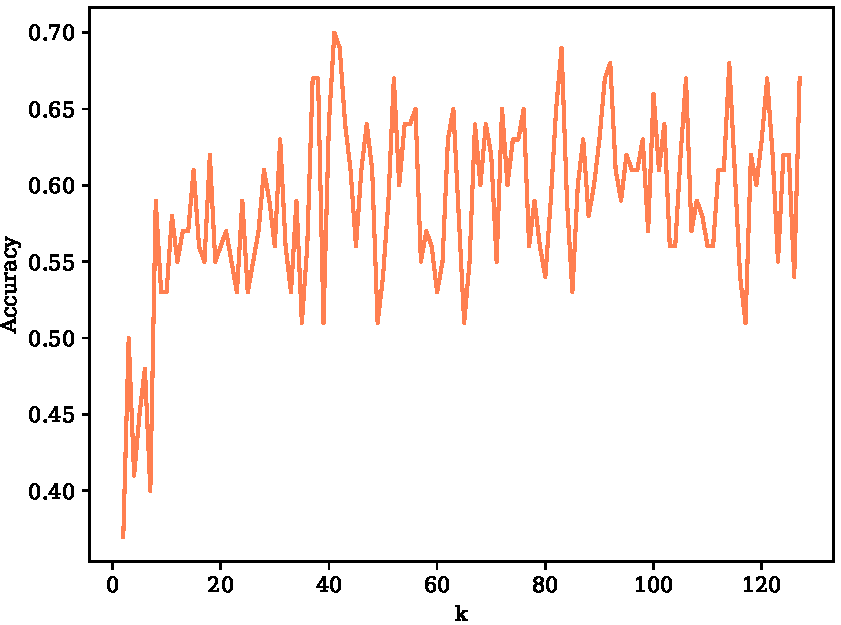
\includegraphics[width=\textwidth]{k_acc.pdf}
          \caption{Accuracy}
          \label{fig:hv_acc}
    \end{subfigure}
    \caption{Results of the experimentation}
    \label{fig:experiment}
\end{figure*}

You can find all the data of the results in the `data/' folder.

